\chapter{Dinamica}
\label{chap:dinamica}

Nel presente capitolo si analizzerà il moto di un corso a partire dai tre principi fondamentali della dinamica fino ad arrivare ad \dots
% Il capitolo non è ancora stato trattato interamente nel corso

\section{I tre principi fondamentali}
    Andiamo ora ad enunciare i tre principi fondamentali della dinamica.
    \begin{law}[Principio d'inerzia]
        In un sistema inerziale, mantiene il suo stato di moto rettilineo uniforme o quiete finché una forza esterna non agisce su questo
    \end{law}
    Da notare come questa legge vale solo ed esclusivamente nel caso nel quale il sistema di riferimento sia inerziale. In caso contrario questo principio \underline{non si applica}.
    \begin{law}[Principio di Newton]
        \label{law:principio-newton}
        L'accelerazione che un corpo riceve è legata a questo mediante una costante numerica $(m)$
    \end{law}
    Quindi $ \vec{a}=m\vec{F}$, spesso la constante $m$ viene apposta al denominatore della formula, ottenendo $ \vec{F}=m\vec{a}$. Questa è la forma più comune della legge di Newton, dove la forza ($F$) è uguale alla massa ($m$)\footnote{Sempre positiva}, misurata in $kg$, per l'accelerazione ($a$) misurata in $m/s^2$.
    \begin{law}[Principio di azione e reazione]
        La forza che un corpo $A$ esercita sul corpo $B$ è uguale alla forza che il corpo $B$ esercita sul corpo $A$, ma di verso opposto.
    \end{law}
    Questo principio è molto importante in quanto ci permette di capire come mai un corpo si muova. Infatti, se un corpo $A$ esercita una forza su un corpo $B$, il corpo $B$ eserciterà una forza uguale e di verso opposto su $A$, l'accelerazione d'altronde sarà diversa se le masse sono diverse.
    \paragraph{Quantità di moto}
        La quantità di moto è una grandezza vettoriale che descrive ``quanto'' movimento c'è in un sistema e dipende dalla massa e dalla velocità del corpo. È definito come segue:
        $$
            \vec{p}=m\vec{v}
        $$
        Ad esempio se un corpo di massa $m=100g$ viaggia a $v=360km/h$ la sua quantità di moto sarà $|\vec{p}|=0.1 [kg] \cdot 100 [m/s] = 10 [kg \cdot m/s]$
    \paragraph{Impulso}
        L'impulso è una grandezza vettoriale che descrive ``quanto'' una forza agisce su un corpo in uno specifico istante/intervallo di tempo. È definito come segue:
        $$
            \vec{J} = \vec{P_f} - \vec{P_i} = \Delta \vec{p} = m_f\vec{v_f} - m_i\vec{v_i}
        $$
        In regime di conservazione della massa, allora $m_f=m_i$ e quindi $\vec{J} = m\vec{v_f} - m\vec{v_i} = m(\vec{v_f} - \vec{v_i}) = m\vec{\Delta v}$ dove $\vec{\Delta v}$ è la variazione di velocità del corpo.\newline
        Inoltre visto il secondo principio (\ref{law:principio-newton}) possiamo scrivere:
        $$
            \vec{F} = m\vec{a} = m\frac{d\vec{v}}{dt} \Rightarrow \vec{F} = m\frac{d\vec{v}}{dt}
        $$
        Questo è anche scrivibile usando la notazione:
        $$
            \vec{F}=m\frac{\Delta \vec{v}}{\Delta t}
        $$
        in questo caso $\vec{J} = \vec{F_{\text{imp}}} \Delta t$ dove $\vec{F_{\text{imp}}}$ è la forza impulsiva, in quanto stiamo trattando di un intervallo di tempo finito e non un infinitesimo.
    \paragraph{Forza risultante}
        La forza risultante è definita come la somma vettoriale di tutte le forze che agiscono su un corpo. $$
            \vec{F_{1\rightarrow c}} + \vec{F_{2\rightarrow c}} + \dots + \vec{F_{N\rightarrow c}} = \sum_{i=1}^{N} \vec{F_{i\rightarrow c}} = \vec{R_{\text{c}}}
        $$
        Dove $\vec{R_{\text{c}}}$ è la forza risultante che agisce sul corpo $c$, mentre $\vec{F_{i\rightarrow c}}$ è la forza che il corpo $i$ esercita sul corpo $c$.\newline
        Se un corpo fosse in quiete ovvero $\vec{S_i} = \vec{S_f}$ dunque $\vec{v_i} = \vec{v_f} = 0$ allora $\vec{a_{tot}} = \vec{0}$ e quindi $\vec{R_{\text{c}}} = \vec{0}$.
\section{Specificazione delle forze}
    \paragraph{Reazione vincolare} La reazione vincolare ($\vec{N}$) è la forza che un corpo esercita su un altro corpo per impedirne il moto. Questa forza è sempre perpendicolare alla superficie di contatto tra i due corpi e diretta verso l'interno del corpo. Questa forza è sempre uguale e di verso opposto alla componente normale della forza peso. Questa forza è detta vincolare in quanto è una forza che impedisce il moto del corpo.
    \paragraph{Forza Peso} La forza peso è la forza che la Terra esercita su un corpo, questa dipende direttamente dalla massa del corpo e dalla costante gravitazionale terrestre $g=9.81 [m/s^2]$. La forza peso è definita come segue: $$
        \vec{P} = m\vec{g}
    $$
    Dunque: $ \vec{F} = m_I \vec{a} = m \vec{g} \Rightarrow \vec{a} = \vec{g} $ possiamo semplificare la massa inerziale con la massa gravitazionale in quando la forza che la terra esercita sulla massa $\vec{F_{M\rightarrow m}} = -\frac{q_{12}q_{21}}{r^2_{12}} \hat{r_{12}} G$ dove $G$ è la costante gravitazionale universale. La formula appena scritta è la formula generale con $q_{12}$ e $q_{21}$ che sono le cariche dei due corpi (quanto un corpo è propenso a partecipare ad una interazione) e $r_{12}$ è la distanza tra i due corpi. Nel caso della forza peso $q_{12}q_{21} = m\cdot M$ dove $M$ è la massa della terra e $m$ è la massa del corpo. Dunque la formula diventa: $$
        \vec{F_{M\rightarrow m}} = -\frac{m\cdot M}{r^2} \hat{r} G
    $$ ora la distanza tra i due corpi è la somma dei raggi dei due corpi, quindi $r = R_{\text{terra}} + h$ dove $R_{\text{terra}}$ è il raggio della terra e $h$ è l'altezza del corpo rispetto al suolo, dato che queste due grandezze sono molto diverse ed $h$ è molto piccolo rispetto a $R_{\text{terra}}$ possiamo approssimare $r \approx R_T$ e quindi la formula diventa: $$
        \vec{F_{M\rightarrow m}} = -\frac{m\cdot M}{R^2} \hat{r} G
    $$
    e quindi $$
        \vec{F_{M\rightarrow m}} = -m\left(\frac{GM}{R^2}\right) \hat{r} = -m\vec{g}
    $$ In quanto questa è una forza allora in un sistema inerziale vale che $\vec{F}=m\vec{a}$ e quindi $m_I\vec{a} = -m\vec{g} \Rightarrow m_I = m$
    \paragraph{Forza Elastica}  
        La forza elastica è la forza che un corpo elastico esercita su un corpo che lo comprime o lo allunga. Questa forza è definita come segue: $$
            \begin{aligned}
                \vec{F_{\text{el}}} =& -k\vec{x}
                =& -k(\vec{x_f} - \vec{x_eq})
            \end{aligned}
        $$
        Dove $k$ è la costante elastica del corpo e $\vec{x}$ è la deformazione del corpo rispetto alla posizione di equilibrio ($\vec{x_{eq}}$). Questa forza è sempre diretta verso la posizione di equilibrio del corpo, dunque se il corpo è compresso la forza sarà diretta verso l'esterno, se il corpo è allungato la forza sarà diretta verso l'interno, in ogni caso il segno meno viene apposto in quanto è in opposizione alla deformazione.
    \paragraph{Forza di Attrito} La forza di attrito è la forza che si oppone al moto di un corpo su una superficie. Questa forza è definita come segue: $$
        \vec{F_{\text{att}}} = -\mu_s|\vec{N}|\cdot \hat{d}
    $$
    Dove $\mu_s$ è il coefficiente di attrito statico, $\vec{N}$ è la reazione vincolare (della quale ne consideriamo il modulo) e $\hat{d}$ è il versore della direzione del moto (dove il segno meno indica che la forza è in opposizione al moto).
    \subsection{Reazione Vincolare}
        Un corpo soggetto alla'azione di una forza, o della risultante non nulla di più forze, rimane fermo allora l'ambiente circostante provoca su quel corpo una forza uguale e di verso opposto alla risultante delle forze che agiscono su di esso, questo in quanto vale la terza legge di Newton. Questa forza è detta \textbf{reazione vincolare} nel caso di un corpo appoggiato su una superficie piana, la reazione vincolare è perpendicolare alla superficie di appoggio e diretta verso l'interno del corpo, opponendosi alla forza peso. La reazione vincolare si indica con $\vec{N}$ e se il corpo è in quiete allora $\vec{R} = \vec{N} + \vec{P} = \vec{0}$.
        \subsubsection{Senzazione di peso} 
            La reazione vincolare esercitata da un corpo, verso un altro corpo, (come un pavimento su una persona) è uguale e di verso opposto alla forza peso. È questa forza che dà la ``sensazione di peso'' e non la forza peso ($P$) in se. Quindi nel caso di un corpo grave appoggiato su una piattaforma orizzontale la quale si muove con accelerazione $a$ allora finché il corpo è appoggiato sulla piattaforma la reazione vincolare sarà $N + P = m\cdot a$, ovvero $N + m\cdot g = m\cdot a$ e quindi $N = m\cdot (a - g)$.\newline
            Questo comporta quattro situazioni differenti:
            \begin{enumerate}
                \item $a$ è discorde con $g$ e (piattaforma accelera verso l'alto) $N$ è maggiore di $P$ e quindi la persona avrà la sensazione di peso maggiore.
                \item $a$ è concorde con $g$ e (piattaforma accelera verso il basso) $N$ è minore di $P$ e quindi la persona avrà la sensazione di peso minore.
                \item $a$ è concorde e coincide esattamente con $g$ allora $N = P$ e quindi la persona avrà la sensazione di assenza di peso.
                \item $a$ è concorde con $g$ allora l'accelerazione sarà così elevata che il corpo ``non riesce a stare dietro'' e quindi ci sarà un distacco tra il corpo e la piattaforma.
            \end{enumerate}
    \subsection{Forza di attrito radente}
        Sperimentalmente si può osservare come se si provi a spingere una massa $m$ su un piano orizzontale, questa non si muoverà per la forza $F$ che si sta esercitando su di essa, ma si muoverà solo nel momento nel quale il modulo della forza $F$ supera un certo valore ($\mu_S N$), il coefficiente $mu_S$ è il coefficiente di attrito statico e questo è dipendente dalle due superfici che si stanno sfregando. Dunque:
        $$
            \begin{cases}
                F\leq \mu_S N & \text{condizione di quiete} \\
                F > \mu_S N & \text{condizione di moto}
            \end{cases}
        $$
        Nel caso in cui il corpo non si muova, la forza di attrito sarà uguale alla forza che si sta esercitando sul corpo, in quanto il corpo non si muove e quindi la forza risultante è nulla. Dunque $F = \mu_S N$ e quindi $N = \frac{F}{\mu_S}$, inoltre la forza di attrito è sempre diretta in opposizione al moto e quindi:
        $$
            R + F + P = 0
        $$
        Chiamiamo $A_{\text{max}}$ il valore massimo di $F$ che possiamo esercitare sul corpo affinché questo non si muova, allora $A_{\text{max}} = \mu_S N$, dove $N$ è la reazione vincolare normale al piano.
        Possiamo quindi disegnare un grafico della forza di attrito in funzione della forza applicata:
        \begin{figure}[H]
            \centering
            \begin{tikzpicture}
                \begin{axis}[
                    axis lines = left,
                    xlabel = $F$,
                    ylabel = $A$,
                    xmin = 0, xmax = 10,
                    ymin = 0, ymax = 10,
                    ytick = {0, 5},
                    yticklabels = {$0$, $A_{\text{max}}$},
                    xtick = {0, 5},
                    xticklabels = {$0$, $F = \mu_S N$},
                ]
                \addplot [
                    domain=0:5, 
                    samples=50, 
                    color=red,
                ]
                {x};
                \addplot [
                    domain=0:10, 
                    samples=100, 
                    color=blue,
                    style=dashed,
                    ]
                {5};
                \end{axis}
            \end{tikzpicture}
            \caption{Grafico della forza di attrito in funzione della forza applicata}
            \label{fig:attritoStatico}
        \end{figure}
        In figura \ref{fig:attritoStatico} possiamo vedere come la forza di attrito sia uguale alla forza applicata fino a quando questa non supera il valore massimo di attrito statico, in quel momento il corpo inizia a muoversi, quando questo accade continua ad esserci attrito ma il corpo si muove e quindi la forza di attrito diventa dinamica.\newline
        La forza che si oppone al movimento di un corpo mentre questo si muove su una superficie è detta forza di attrito radente dinamico, questa forza è definita come segue:
        $$
            F_{\text{ad}} = -\mu_d N = ma
        $$
        Dove $\mu_d$ è il coefficiente di attrito dinamico, $N$ è la reazione vincolare. Dalla definizione notiamo come la forza di attrito dinamico sia sempre diretta in opposizione al moto ed \underline{non è affetta dalla velocità del corpo}, possiamo quindi aggiungere al grafico della Figura \ref{fig:attritoStatico} la forza di attrito dinamico:
        \begin{figure}[H]
            \centering
            \begin{tikzpicture}
                \begin{axis}[
                    axis lines = left,
                    xlabel = $F$,
                    ylabel = $A$,
                    xmin = 0, xmax = 10,
                    ymin = 0, ymax = 10,
                    ytick = {0, 4.75, 5},
                    yticklabels = {$0$, $A_{\text{d}}$, $A_{\text{max}}$},
                    xtick = {0, 5},
                    xticklabels = {$0$, $F = \mu_S N$},
                ]
                \addplot [
                    domain=0:5, 
                    samples=50, 
                    color=red,
                ]
                {x};
                \addplot [
                    domain=0:10, 
                    samples=100, 
                    color=blue,
                    style=dashed,
                    ]
                {5};
                \addplot[
                    domain=5:5.25,
                    samples=50,
                    color=red,
                ]{1/((x-3.95)^21+1)+4.75};
                \addplot [
                    domain=5.25:10, 
                    samples=50, 
                    color=red,
                    ]
                {4.75};
                \end{axis}
            \end{tikzpicture}
            \caption{Grafico della forza di attrito in funzione della forza applicata}
            \label{fig:attritoDinamico}
        \end{figure}
        Notiamo come il valore di $A_{\text{d}}$ sia minore di $A_{\text{max}}$ in è vero per ogni superficie che il coefficiente di attrito dinamico sia minore di quello statico ($\mu_d < \mu_S$), altrimenti il corpo non si muoverebbe.
    \subsection{Piano Inclinato}
        Se prendiamo in considerazione un corpo di massa $m$ assimilabile ad un punto materiale e soggetto alle forze peso, reazione vincolare e forza di attrito radente, se questo è appoggiato su una superficie inclinata di angolo $\theta$ rispetto all'orizzontale, allora se è la sola forza peso che agisce sul corpo, allora possiamo scrivere la seguente equazione:
        $$
            P + R = m\cdot a
        $$
        Dove $P$ è la forza peso, $R$ è la reazione vincolare e $a$ è l'accelerazione del corpo, la reazione vincolare agisce solo nella direzione normale alla superficie, quindi possiamo scomporre questo come:
        $$
            \begin{cases}
                -mg\cos \theta + N = 0 & \text{direzione normale} \\
                -mg\sin \theta = m\cdot a & \text{direzione parallela}
            \end{cases}
        $$
        Da queste due equazioni possiamo notare come tutta l'eventuale accelerazione del corpo sia diretta lungo la superficie inclinata.\footnote{Ancora non abbiamo preso in considerazione la forza di attrito radente}
        \begin{figure}[H]
            \centering
            % Figura di un corpo su un piano inclinato (triangolo rettangolo (angolo retto in basso a sinistra)  con la punta di angolo in basso a destra) con la forza peso, la suddivisione delle forze peso in due componenti, la reazione vincolare, il corpo è un rettangolo appoggiato sul piano inclinato. Gli angoli tra le componenti della forza peso e il piano inclinato devono essere indicati.
            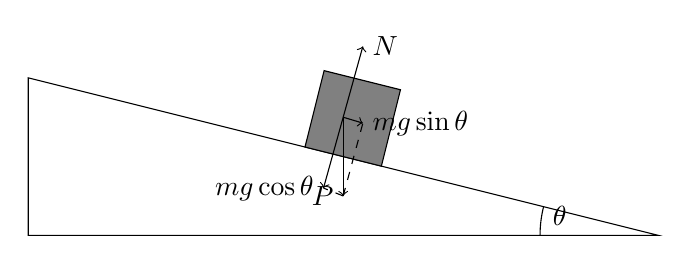
\begin{tikzpicture}
                % Piano inclinato
                \draw (0,0) -- (8,0) -- (0,2) -- cycle;
                % Angoli del piano inclinato
                \draw (6.5,0) arc (180:166.15:1.5);
                \node at (6.75,0.25) {$\theta$};

                % Corpo appoggiato sul piano inclinato
                \draw[fill=gray, rotate around={-14.04:(4,1)}] (3.5,2) rectangle (4.5,1);
                % Forza peso
                \draw[->] (4,1.5) -- (4,0.5) node[anchor=east] {$P$};
                % Componenti della forza peso
                \draw[->] (4,1.5) -- (3.75,0.6) node[anchor=east] {$mg\cos \theta$};
                \draw[->] (4,1.5) -- (4.25,1.425) node[anchor=west] {$mg\sin \theta$};
                % Linee tratteggiate di supporto
                \draw[dashed] (4,0.5) -- (3.75,0.6);
                \draw[dashed] (4,0.5) -- (4.25,1.425);
                % Reazione vincolare
                \draw[->] (4,1.5) -- (4.25,2.4) node[anchor=west] {$N$};
            \end{tikzpicture}
            \caption{Forze che agiscono su un corpo su un piano inclinato}
            \label{fig:pianoInclinato}
        \end{figure}
        Ora, prendendo in considerazione anche la forza di attrito radente, distinguiamo due principali casi:
        \begin{itemize}
            \item Il corpo è in stasi rispetto al piano inclinato
            \item Il corpo sta scendendo (frenato) rispetto al piano inclinato
        \end{itemize}
        Nel primo caso ciò significa che la forza di attrito statico è uguale alla componente parallela della forza peso, quindi $F_{\text{att}} = \mu_S N = mg\sin \theta$ ed inoltre questa non eccede il valore massimo di attrito statico, quindi $\mu_S N \leq \mu_S mg\cos \theta$, dunque $mg\sin \theta = \mu_S mg\cos \theta$ e quindi $ mg(\sin \theta - \mu_S \cos \theta) = 0$ e quindi $\mu_S \geq \tan \theta$.\newline
        Nel secondo caso, il corpo sta scendendo rispetto al piano inclinato, quindi viene esercitata una forza di attrito dinamico, questa forza è minore della componente parallela della forza peso, il corpo scende con accelerazione $a$ e quindi $mg\sin \theta - F_{\text{att}} = m\cdot a$ e quindi $mg\sin \theta - \mu_d N = m\cdot a$ e quindi $mg\sin \theta - \mu_d mg\cos \theta = m\cdot a$ e quindi $a = g(\sin \theta - \mu_d \cos \theta)$.

    \subsection{Forza Elastica - senza attrito}
        Se prendiamo in considerazione un corpo di massa $m$ ancorato ad una molla la quale a sua volta è ancorata ad un muro, allora quando il corpo viene allontanato dalla posizione di equilibrio della molla, questa eserciterà una forza elastica sul corpo, questa forza è definita come segue:
        $$
            \vec{F}=-k\vec{x}=m\vec{a}\Rightarrow -k\vec{x} = m\frac{d^2\vec{x}}{dt^2}
        $$
        Dove $k$ è la costante elastica della molla, $\vec{x}$ è la deformazione della molla rispetto alla posizione di equilibrio e $\vec{a}$ è l'accelerazione del corpo secondo la seconda legge di Newton. La forza elastica è sempre diretta verso la posizione di equilibrio della molla, quindi se il corpo è compresso la forza sarà diretta verso l'esterno, se il corpo è allungato la forza sarà diretta verso l'interno, in ogni caso il segno meno viene apposto in quanto è in opposizione alla deformazione.
        \begin{figure}[H]
            \centering
            \begin{tikzpicture}
                \def\H{1.1}  % wall height
                \def\T{0.3}  % wall thickness
                \def\W{3.9}  % ground length
                \def\D{0.25} % ground depth
                \def\h{0.7}  % mass height
                \def\w{0.8}  % mass width
                \def\x{2.0}  % mass x position
                \def\dx{0.8} % extension
                \def\y{1.22*\H} % x axis y position
                \def\F{0.8}  % force
                
                % AXIS
                \draw[mydashed] (\x,0) --++ (0,\y) (\x+\dx,0) --++ (0,1.1*\y);
                \draw[axis] (\x-0.4*\W,\y) -- (\x+0.4*\W,\y) node[right] {$x$};
                \tick{\x,\y}{-90} node[scale=0.8,above=-1] {$0$};
                \draw[ell] (0,1.3*\h) --++ (\x,0) node[midway,fill=white,inner sep=0] {$\ell_0$};
                \draw[dx] (\x,1.6*\h) --++ (\dx,0) node[pos=0.45,fill=white,inner sep=0] {$x$};
                
                % SPRING & MASS
                \draw[spring,segment length=7.5] (0,\h/2) --++ (\x+\dx,0);
                \draw[ground] (0,0) |-++ (-\T,\H) |-++ (\T+\W,-\H-\D) -- (\W,0) -- cycle;
                \draw (0,\H) -- (0,0) -- (\W,0);
                \draw[mass] (\x+\dx,0) rectangle++ (\w,\h) node[midway] {$m$};
                \draw[force] (\x+\dx+0.2*\w,0.9*\h) --++ (-\F,0) node[midway,right=1,above=-1] {$\vb{F}$};
                
            \end{tikzpicture}
            \caption{Diagramma di un corpo su una molla senza attrito}
        \end{figure}
        Dall'ultima equazione possiamo notare come questa possa essere scritta come:
        $$
            m\frac{d^2\vec{x}}{dt^2}=-k\vec{x} \Rightarrow \frac{d^2\vec{x}}{dt^2}+\frac{k}{m}\vec{x}=0
        $$
        Dal quale possiamo definire $\omega$ ovvero ``la pulsazione'' come:
        \begin{align}
            \omega^2 \stackrel{\text{def.}}{\rightharpoonup} \frac{k}{m} \Rightarrow \omega = \sqrt{\frac{k}{m}} \label{eq:omega}
        \end{align}
        Inoltre in quando $\vec{x}=x\hat{x}$ ed il verso ($\hat{x}$) è costante, possiamo scrivere:
        \begin{align}
            \vec{x} \longrightarrow x \label{eq:posizione}
        \end{align}
        Ora viste le due equazioni (\ref{eq:omega}) e (\ref{eq:posizione}) possiamo scrivere:
        $$
            \frac{d^2x}{dt^2}+\omega^2 x = 0 \Longrightarrow \ddot{x}+\omega^2 x = 0 
        $$
        Questa è l'equazione differenziale del moto armonico semplice, la quale ha come soluzione:
        $$
            x(t) = A\cos(\omega t + \phi) \label{eq:soluzione}
        $$
        Abbiamo già incontrato i parametri $A$ e $\phi$ quando abbiamo parlato di moto armonico semplice, questi hanno lo stesso ruolo in questo caso, ovvero $A$ è l'ampiezza del moto e $\phi$ è la fase iniziale del moto.\newline
        Questo moto ci suggerisce che, in assenza di attrito, la molla non termina mai il suo moto, ma continua a vibrare indefinitamente con una frequenza angolare $\omega$ e un'ampiezza $A$, che è la distanza massima dalla posizione di equilibrio. 
        \begin{figure}[H]
            \centering
            \begin{tikzpicture}
                \def\A{1.0} % ampiezza
                \def\T{2.0} % periodo
                \begin{axis}[
                    axis lines = left,
                    xlabel = $t$,
                    ylabel = $x$,
                    xmin = 0, xmax = \T+0.5,
                    ymin = -\A-0.5, ymax = \A+0.5,
                    xtick = {0, \T/4, \T/2, 3*\T/4, \T},
                    xticklabels = {$0$, $\frac{T}{4}$, $\frac{T}{2}$, $\frac{3T}{4}$, $T$},
                    ytick = {-\A, -\A/2, 0, \A/2, \A},
                    yticklabels = {$-A$, $-\frac{A}{2}$, $0$, $\frac{A}{2}$, $A$},
                    samples=100,
                    smooth,
                ]
                \addplot [
                    color=red,
                    domain=0:\T+0.5,
                ]{(\A)*cos(deg(2*pi*x/\T))};
                \end{axis}
            \end{tikzpicture}
            \caption{Grafico del moto armonico semplice}
            \label{fig:motoArmonicoSemplice}
        \end{figure}
        In figura \ref{fig:motoArmonicoSemplice} possiamo vedere il grafico del moto armonico semplice, dove $A$ è l'ampiezza del moto e $T$ è il periodo del moto. Vista l'equazione del moto il parametro $A$ è calcolato come: $$
            A = \sqrt{x^2_0 + \frac{v_0^2}{\omega^2}} \label{eq:ampiezza}
        $$
        Dove $x_0$ è la posizione iniziale del corpo e $v_0$ è la velocità iniziale del corpo, se questo è in quiete allora $v_0 = 0$ e quindi $A = x_0$.
    \subsection{Moto del pendolo}
        Per come viene affrontato il moto del pendolo all'interno di questo corso si considerino le seguenti ipotesi:
        \begin{itemize}
            \item Non sono presenti attriti nel filo
            \item Il filo è inestensibile
            \item Il filo non ha massa
            \item La massa del pendolo è concentrata in un punto materiale
            \item Il pendolo non è soggetto alla resistenza dell'aria
            \item Il pendolo è situato nel vuoto
            \item Il pendolo è soggetto alla forza di gravità costante ($g$) e uniforme
        \end{itemize}
        Una volta definite queste ipotesi possiamo passare a definire il moto del pendolo. Il pendolo è un sistema composto da una massa $m$ appesa ad un filo di lunghezza $L$, il quale è fissato ad un punto di sospensione.\newline
        Se il pendolo è in quiete, la forza peso $P$ agisce verticalmente verso il basso e la reazione vincolare $N$ agisce lungo il filo.
        
        \begin{figure}[H]
            \centering
            \begin{tikzpicture}
                % save length of g-vector and theta to macros
                \pgfmathsetmacro{\Gvec}{1.5}
                \pgfmathsetmacro{\myAngle}{0}
                % calculate lengths of vector components
                \pgfmathsetmacro{\Gcos}{\Gvec*cos(\myAngle)}
                \pgfmathsetmacro{\Gsin}{\Gvec*sin(\myAngle)}
                
                \coordinate (centro) at (0,0);
                \draw[dashed,gray,-] (centro) -- ++ (0,-3.5) node (mary) [black,below]{$ $};
                \draw[thick] (centro) -- ++(270+\myAngle:3) coordinate (bob);
                \draw [blue,-stealth] (bob) -- ($(bob)!\Gcos cm!(centro)$);
                \draw [-stealth] (bob) -- ++(0,-\Gvec)
                    coordinate (g)
                    node[near end,left] {$g$};
                \filldraw [fill=black!40,draw=black] (bob) circle[radius=0.1];
            \end{tikzpicture}
            \caption{Schema delle forze che agiscono su un pendolo sulla verticale}
        \end{figure}

        Se invece il pendolo è in movimento, la forza peso $P$ agisce comunque verso il basso, la tensione del filo $T_f$ agisce lungo questo ed il pendolo è in movimento dunque per la seconda legge di Newton possiamo scrivere:
        $$
            P + T_f = m\cdot a \Rightarrow m\cdot g + T_f = m\cdot a
        $$
        Possiamo scomporre le forze in due componenti, una normale alla direzione del pendolo e una parallela alla direzione del pendolo, in questo modo possiamo scrivere:
        $$
            \begin{aligned}
                N: \quad & -T_f + P_\perp & = 0\\
                \tau: \quad & -P_\parallel & = m\cdot a_\tau
            \end{aligned} = \begin{cases}
                -T_f + m\cdot g\cdot \cos \theta &= 0 \\
                \cancel{m}\cdot g\cdot \sin \theta &= \cancel{m}\cdot a_\tau
            \end{cases} = 
            \begin{cases}
                T_f &= m\cdot g\cdot \cos \theta \\
                a_\tau &= g\cdot \sin \theta
            \end{cases}
        $$
        \begin{figure}[H]
            \centering
            \begin{tikzpicture}
                % save length of g-vector and theta to macros
                \pgfmathsetmacro{\Gvec}{1.5}
                \pgfmathsetmacro{\myAngle}{30}
                % calculate lengths of vector components
                \pgfmathsetmacro{\Gcos}{\Gvec*cos(\myAngle)}
                \pgfmathsetmacro{\Gsin}{\Gvec*sin(\myAngle)}
            
                \coordinate (centro) at (0,0);
                \draw[dashed,gray,-] (centro) -- ++ (0,-3.5) node (mary) [black,below]{$ $};
                \draw[thick] (centro) -- ++(270+\myAngle:3) coordinate (bob);
                \pic [draw, ->, "$\theta$", angle eccentricity=1.5] {angle = mary--centro--bob};
                \draw [blue,-stealth] (bob) -- ($(bob)!\Gcos cm!(centro)$);
                \draw [-stealth] (bob) -- ($(bob)!-\Gcos cm!(centro)$)
                    coordinate (gcos)
                    node[midway,above right] {$a\cos\theta$};
                \draw [-stealth] (bob) -- ($(bob)!\Gsin cm!90:(centro)$)
                    coordinate (gsin)
                    node[midway,above left] {$a\sin\theta$};
                \draw [-stealth] (bob) -- ++(0,-\Gvec)
                    coordinate (g)
                    node[near end,left] {$g$};
                \pic [draw, ->, "$\theta$", angle eccentricity=1.5] {angle = g--bob--gcos};
                \filldraw [fill=black!40,draw=black] (bob) circle[radius=0.1];
            \end{tikzpicture}
            \caption{Schema delle forze che agiscono su un pendolo non sulla verticale}
        \end{figure}
        Dunque la tensione del filo al momento del rilascio del pendolo è uguale alla componente normale della forza peso, mentre l'accelerazione tangenziale è uguale alla componente tangenziale della forza peso. Queste però valgono solo se il pendolo è appena stato rilasciato, infatti nel momento in cui il pendolo inizia a muoversi esiste una ``forza di richiamo'' che ``tenta'' di riportare il pendolo alla posizione di equilibrio, questa forza, a differenza della molla, non ha una direzione costante, ma cambia in funzione dell'angolo $\theta$ e della lunghezza del pendolo $L$. Dunque nei momenti successivi al rilascio del pendolo, possiamo scomporre le forze come:
        $$
            \left\{
                \begin{aligned}
                    -T + P_\perp &= m\cdot a_n
                    P_\parallel &= m\cdot a_\tau
                \end{aligned}
            \right.
            \Rightarrow \left\{
                \begin{aligned}
                    -T + m\cdot g\cdot \cos \theta &= m\cdot a_n \\
                    m\cdot g\cdot \sin \theta &= m\cdot a_\tau
                \end{aligned}
            \right.
            \Rightarrow \left\{
                \begin{aligned}
                    -\frac{T}m+g\cdot \cos \theta &= a_n \\
                    g\cdot \sin \theta &= a_\tau
                \end{aligned}
            \right.
        $$
        Per esprimere la forza di richiamo in funzione dell'angolo $\theta$ e della lunghezza del pendolo $L$, possiamo scrivere:
        $$
            \begin{aligned}
                a_t &= \frac{R d^2\theta}{dt^2} = \frac{l d^2 v}{dt^2}\\
                a_n &= \frac{v^2}{R} = \frac{v^2}{l}=\frac1l\left(\frac{ds}{dt}\right)^2 = \frac{1}{l}\left(\frac{d\theta}{dt}\right)^2 = \frac{l^{\cancel{2}}}{\cancel{l}} \left(\frac{d\theta}{dt}\right)^2 = l\left(\frac{d\theta}{dt}\right)^2
            \end{aligned}
        $$
        Invertendo opportunamente i versi del sistema di riferimento possiamo scrivere: $$
            \left\{
                T_f - P_\perp = m a_n = m\frac{v^2}l\\
                -P_\parallel = m a_\tau = m\frac{d^2\theta}{dt^2}
            \right.
        $$
        Ora come visto in precedenza la tensione del filo dipende dall'angolo $\theta$, $\tau(\theta)=mg\cos \theta + m\frac{v^2(\theta)}l$ dunque possiamo scrivere:
        $$
            -\cancel{m}g\sin \theta = \cancel{m}\frac{d^2\theta}{dt^2} \Rightarrow \frac{d^2\theta}{dt^2} + \frac{g}{l}\sin \theta = 0
        $$
        Il che significa che la massa del pendolo non influisce sul moto del pendolo, ma solo la lunghezza del pendolo e l'accelerazione di gravità. Questa è l'equazione differenziale del moto armonico semplice, la quale ha come soluzione:
        $$
            \ddot{v}+\frac{g}{l}\sin \theta = 0
        $$
        Ora risolvere per ogni valore di $\theta$ è difficile!
        \subsubsection{Piccole oscillazioni}
            Prendiamo ora in considerazione un angolo $\theta$ molto piccolo ($\theta \ll 1$), in questa situazione vale che:
            $$
                \sin \theta \leq \theta \leq \tan \theta
            $$
            per lo sviluppo in serie di Taylor vale che:
            $$  
                \sin \theta \approx \theta - \frac{\theta^3}{6} + O(\theta^5)
            $$
            Si hanno correzioni nell'ordine di $\theta^3$, ma per $\theta$ molto piccolo ($\theta = 0.17 \Rightarrow \theta^3 = 0.005$) possiamo considerare $\sin \theta \approx \theta$, quindi possiamo scrivere:
            $$
                \ddot{v}+\frac{g}{l}\theta = 0 \Rightarrow \ddot{v}+\omega\theta = 0
            $$
            Dove $\omega = \sqrt{\frac{g}{l}}$ è la pulsazione del pendolo. Questa ci dice che per $\theta$ molto piccolo il periodo non dipende dall'angolo $\theta$, ma solo dalla lunghezza del pendolo e dall'accelerazione di gravità, dunque siamo in situazione di \textbf{ISOCRONISMO}.